\subsection{Problema dell'esplorazione} \label{subsec:prob_esplorazione}
Si consideri una regione in cui sono presenti alcuni elementi, ma di cui non si conoscono alcune informazioni; per esempio le posizioni degli utenti e il loro numero in un determinato istante di tempo.
Ci si pone quindi il problema di come, utilizzando le stesse fonti di segnale utilizzate per il problema di copertura, esplorare le porzioni di regione che in un determinato istante non sono coperte dal segnale della rete.

Come per la copertura, in ambito scientifico si vanno ad individuare due categorie di algoritmi per l'esplorazione di un'area: algoritmi statici, in cui si determina a priori il percorso che un agente deve percorrere affinché ogni zona della regione venga esplorata almeno una volta, pensati per contesti in cui l'ambiente non varia o le cui variazioni sono sufficientemente lente, e algoritmi dinamici, in cui invece l'esplorazione di una zona potrebbe ripetersi più volte nel tempo, al seguito della variazione di alcune condizioni (Figura \ref{fig:path_static_dynamic_environment}).

\begin{figure}[ht]
    \centering
    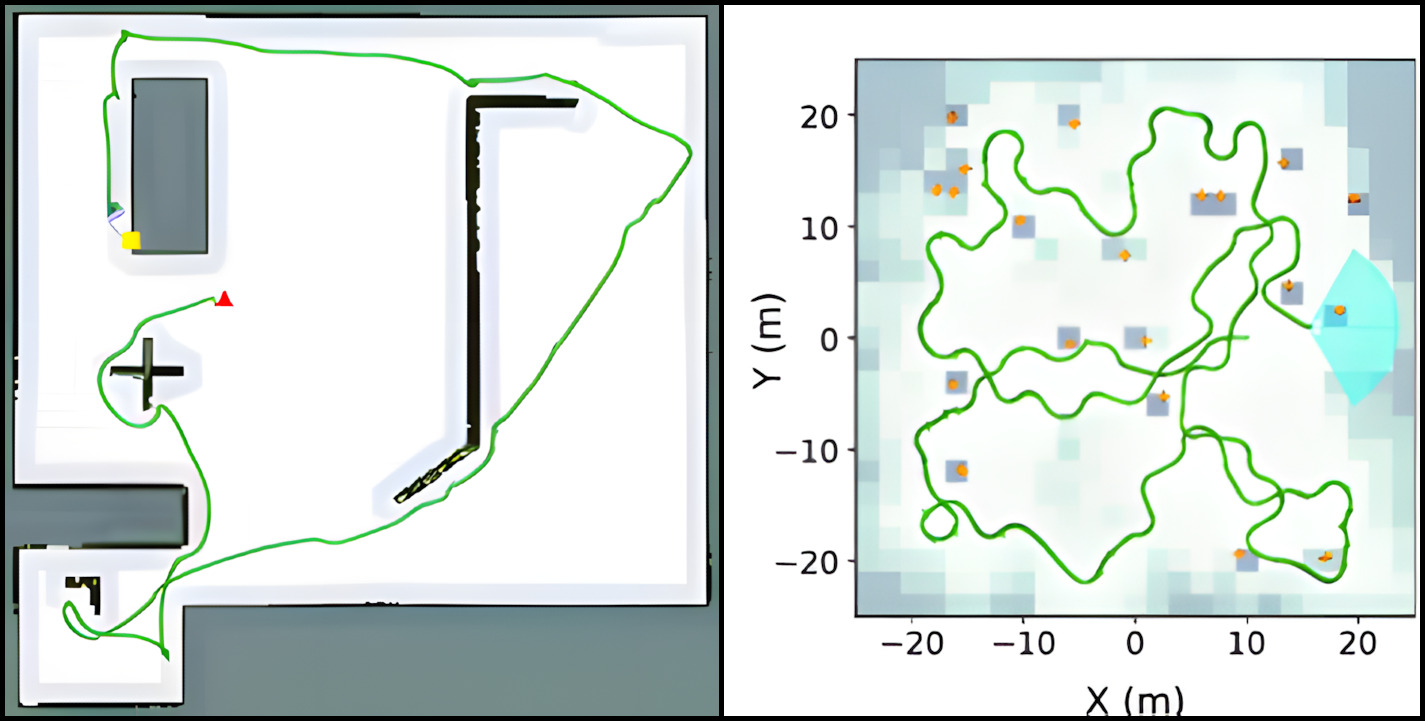
\includegraphics[width=0.9\textwidth]{img/ch1/path_dynamic_static_environment.jpg}
    \caption[Esempi di traiettorie in ambiente statico e dinamico]{Esempi di traiettorie in un processo di esplorazione: a sinistra,ù in ambiente statico; a destra in ambiente dinamico. Si osserva come l'ambiente dinamico provoca una traiettoria molto più caotica.}
    \label{fig:path_static_dynamic_environment}
\end{figure}
\pagebreak
In questa tesi si affronterà un problema in cui l'ambiente da esplorare verrà considerato dinamico, e quindi verrà adottato un algoritmo di esplorazione da eseguire ripetutamente nel tempo.
Si suppone infatti che all'interno della regione di interesse le posizioni degli utenti non siano note, e che il numero degli stessi possa variare: un nuovo utente quindi, posizionato in una zona già visitata ma non attualmente coperta, potrebbe richiedere la connessione alla rete, oppure un utente già presente e coperto potrebbe disconnettersi dalla rete.
